\chapter{Swarm Intelligence (SI)}




\section{Motivation}
    In real world most of time we aren't simply working with just one robot. Indeed many a time, several robots have to cooperate to do some task. For the same reason we want to study the behaviour of robots when they will be working together. This is swarm behaviour. Lets understand it in more depth as below. 



\section{Introduction}
Swarm intelligence is the collective behavior of decentralized, self-organized systems, natural or artificial. The concept is employed in work on artificial intelligence.\cite{SwarmIntelligence}
SI systems consist typically of a population of simple agents interacting locally with one another and with their environment. The inspiration often comes from nature, especially biological systems. The agents follow very simple rules, and although there is no centralized control structure dictating how individual agents should behave, local, and to a certain degree random, interactions between such agents lead to the emergence of "intelligent" global behavior, unknown to the individual agents. Examples of swarm intelligence in natural systems include ant colonies, bird flocking, hawks hunting, animal herding, bacterial growth, fish schooling and microbial intelligence.\cite{SwarmBehaviour}


\section{Example of swarm behaviour}
\subsection{Foraging}
Foraging is searching for food resources. A group of birds/animals can make their search for food efficient by adopting some common behaviour(will explain below in detail). Their behaviour will help the group as whole sustain their life.\cite{Foraging}

\subsection{Flocking}
Flocking behavior is the behavior exhibited when a group of birds, called a flock, are foraging or in flight. It is when, several birds fly in group for their common advantage e.g. protection from predator.

\subsection{Schooling}
It is similar to flocking but for fishes.

\subsection{Ant Colony}
In ant colony, when group of ant found a food source then always tend to travel to/fro from it to their home in shortest path possible. This possible because secretes/put a chemical on the path when move through it. Eventually, shortest path tend to get more of this chemical and hence ant always follow the shortest path.



\section{Algorithms}

\subsection{Particle swarm optimization (PSO)}
PSO is a computational method that optimizes a problem by iteratively trying to improve a candidate solution with regard to a given measure of quality. It solves a problem by having a population of candidate solutions, here dubbed particles, and moving these particles around in the search-space according to simple mathematical formulae over the particles position and velocity. Each particles movement is influenced by its local best known position, but is also guided toward the best known positions in the search-space, which are updated as better positions are found by other particles. This is expected to move the swarm toward the best solutions.\cite{PSO}


A basic variant of the PSO algorithm works by having a population of particles. These particles are moved around in the search-space according to a few simple formulae. The movements of the particles are guided by their own best known position in the search-space as well as the entire swarms best known position. When improved positions are being discovered these will then come to guide the movements of the swarm. The process is repeated and by doing so it is hoped, but not guaranteed, that a satisfactory solution will eventually be discovered.\cite{PSO}


\subsubsection{Pseudo Code}
\begin{minted}{python}
 '''
 Let f: Rn -> R be the cost function which must be minimized. The function takes a candidate solution as an argument in the form of a vector of real numbers and produces a real number as output which indicates the objective function value of the given candidate solution. The gradient of f is not known. The goal is to find a solution a for which f(a) <= f(b) for all b in the search-space, which would mean a is the global minimum.

Let S be the number of particles in the swarm, each having a position xi belongs to Rn in the search-space and a velocity vi belongs to Rn. Let pi be the best known position of particle i and let g be the best known position of the entire swarm. A basic PSO algorithm is then:
 '''
 
 
 for each particle i = 1, ..., S do
   Initialize the particles position with a uniformly distributed random vector(xi)
   Initialize the particles best known position to its initial position(pi)
   if f(pi) < f(g) then
       update the swarms best known  position(g)
   Initialize the particles velocity
   
while a termination criterion is not met do:
   for each particle i = 1, ..., S do
      for each dimension d = 1, ..., n do
         Update the particles velocity(vi)
      Update the particles position: xi <- xi + vi
      if f(xi) < f(pi) then
         Update the particles best known position: pi <- xi
         if f(pi) < f(g) then
            Update the swarms best known position: g <- pi
            
\end{minted}



\subsection{Flocking}
In the natural world, organisms exhibit certain behaviors when traveling in groups. This phenomenon, also known as flocking, occurs at both microscopic scales (bacteria) and macroscopic scales (fish). Using computers, these patterns can be simulated by creating simple rules and combining them. This is known as emergent behavior, and can be used in games to simulate chaotic or life-like group movement.\cite{WikiFlocking}

Basic models of flocking behavior are controlled by three simple rules:
    \begin{enumerate}
        \item \textbf{Separation} - avoid crowding neighbours (short range repulsion)
        \item \textbf{Alignment} - steer towards average heading of neighbours
        \item \textbf{Cohesion} - steer towards average position of neighbours (long range attraction)
    \end{enumerate}

\newline \begin{figure}[H]
    \centering
    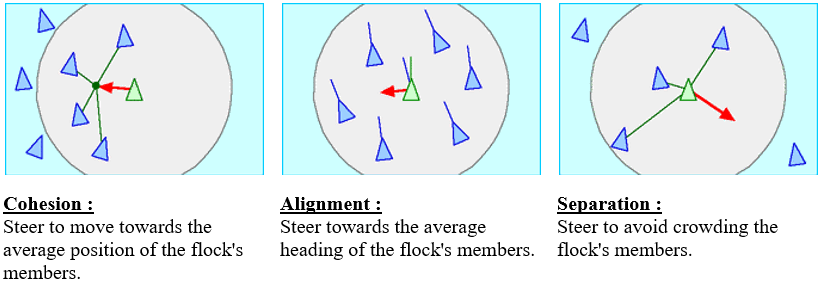
\includegraphics[width=1.0\textwidth]{images/flock.png}
    \caption{Flocking rules}
\end{figure}

With these three simple rules, the flock moves in an extremely realistic way, creating complex motion and interaction that would be extremely hard to create otherwise.

\section{Implementation}
\subsection{Particle swarm optimization (PSO)}
We use the PSO algorithm(described above) to solve some basis problem.
\begin{figure}[H]
    \centering
    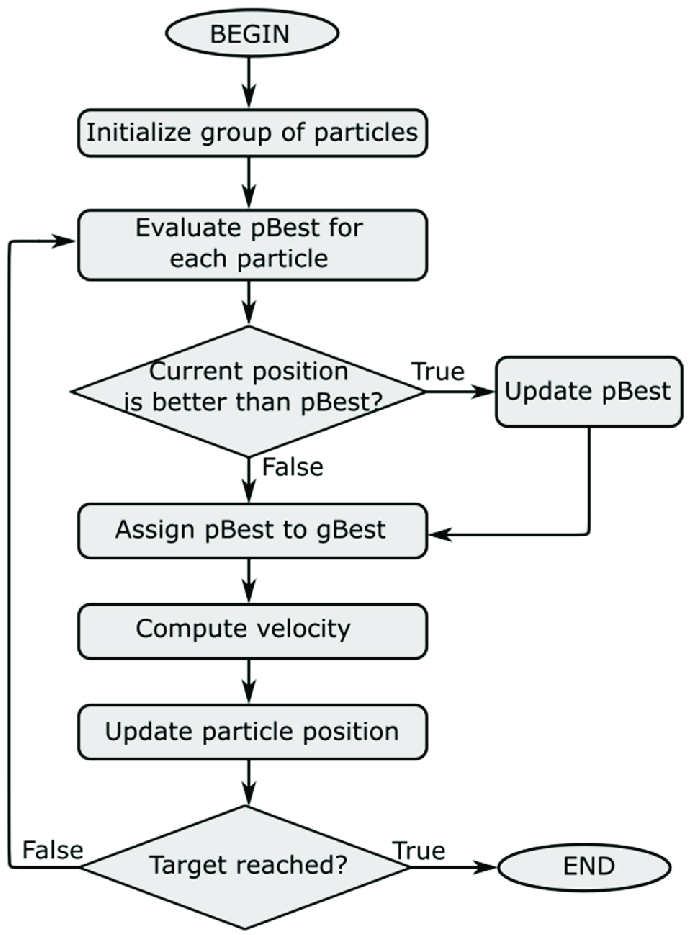
\includegraphics[width=0.6\textwidth]{images/psoflowchart.png}
    \caption{PSO flow chart}
\end{figure}
\subsubsection{Finding the global minimum of function}
Here I created python class for particle and environment. Multiple particle altogether tries to find the minimum value of the given function. Here function is \[ cost = x^n + y^n + 1 \] here x and y are coordinate of the particles. Hence origin with be the only minima. Particle finds this point by cooperating in best possible way by follow PSO algorithm. Detailed code of the same can be found \href{https://github.com/iamrajee/Slam_and_RL_BTP/tree/master/code/swarm/pso}{here}.
\subsubsection{Pseudo code}
\begin{minted}{python}
Run for n iterations:
    # update personal and global best
    for ith particle:
        fitness_cadidate = fitness_function(particle_position_vector[i])
        
        # Personal update 
        if(pbest_fitness_value[i] > fitness_cadidate):
            pbest_fitness_value[i] = fitness_cadidate
            pbest_position[i] = particle_position_vector[i]
        
        # global update 
        if(gbest_fitness_value > fitness_cadidate):
            gbest_fitness_value = fitness_cadidate
            gbest_position = particle_position_vector[i]
    
    
    #break if required constrained met
    if(abs(gbest_fitness_value - target) < target_error):
        break
    
    
    # calculate new velocity and hence new position for each particle
    for ith particle:
        # update velocity
        new_velocity = (W*velocity_vector[i]) + (c1*random.random()) * (pbest_position[i] - particle_position_vector[i]) + (c2*random.random()) * (gbest_position-particle_position_vector[i])
        
        # update position
        new_position = new_velocity + particle_position_vector[i]
        particle_position_vector[i] = new_position
    iteration++
\end{minted}


\newline \begin{figure}[H]
    \centering
    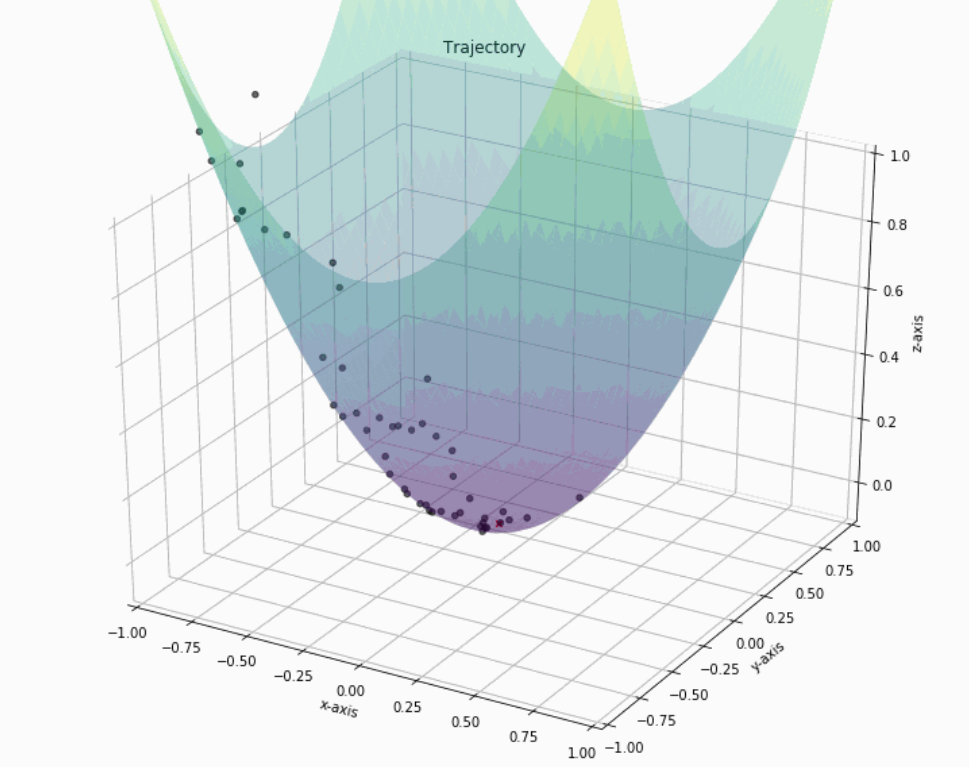
\includegraphics[width=0.5\textwidth]{images/pso3.png}
    \caption{PSO : Random initialisation of particles}
\end{figure}
\newline \begin{figure}[H]
    \centering
    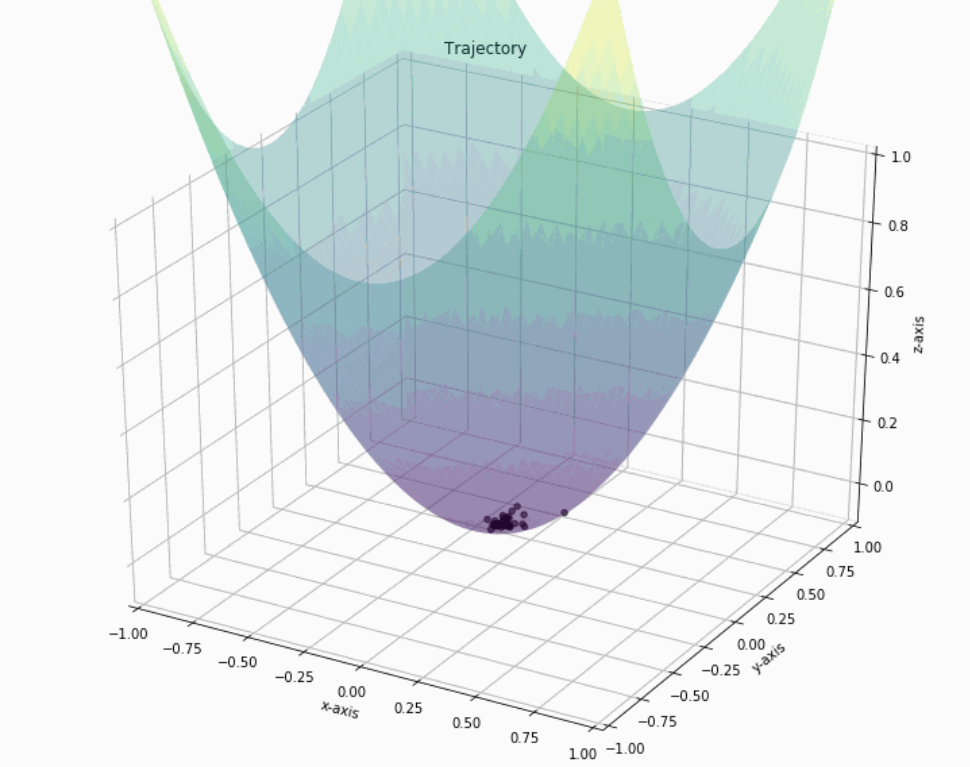
\includegraphics[width=0.5\textwidth]{images/pso4.png}
    \caption{PSO : Particles converging to global minima}
\end{figure}
\newline \begin{figure}[H]
    \centering
    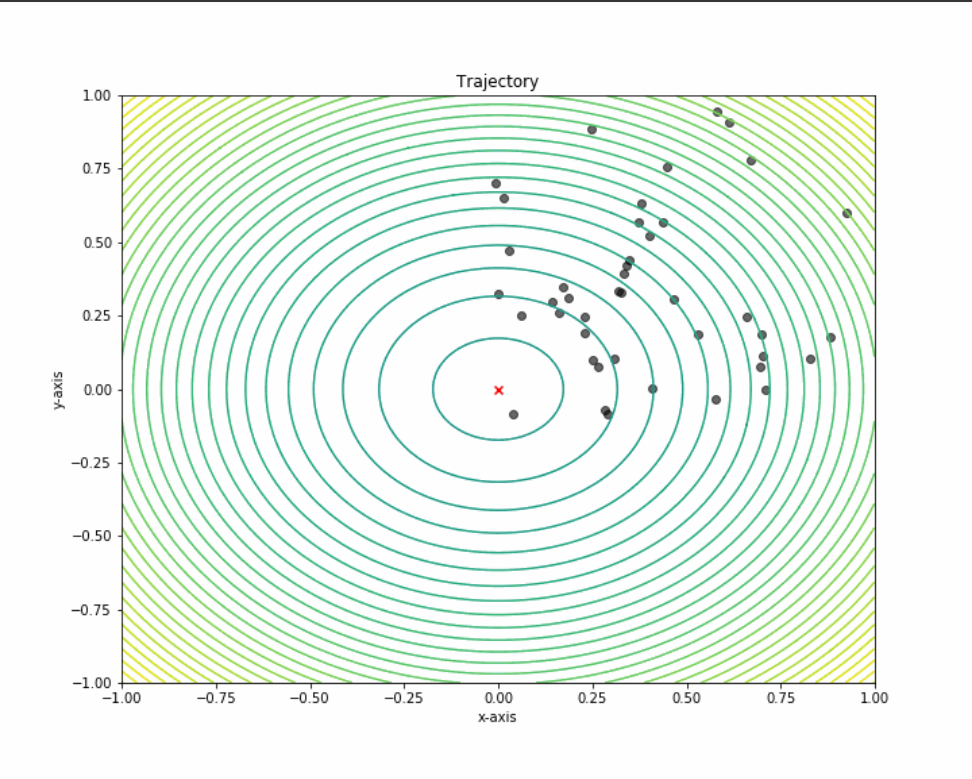
\includegraphics[width=0.5\textwidth]{images/pso1.png}
    \caption{PSO : Random initialisation of particles(Top view)}
\end{figure}
\newline \begin{figure}[H]
    \centering
    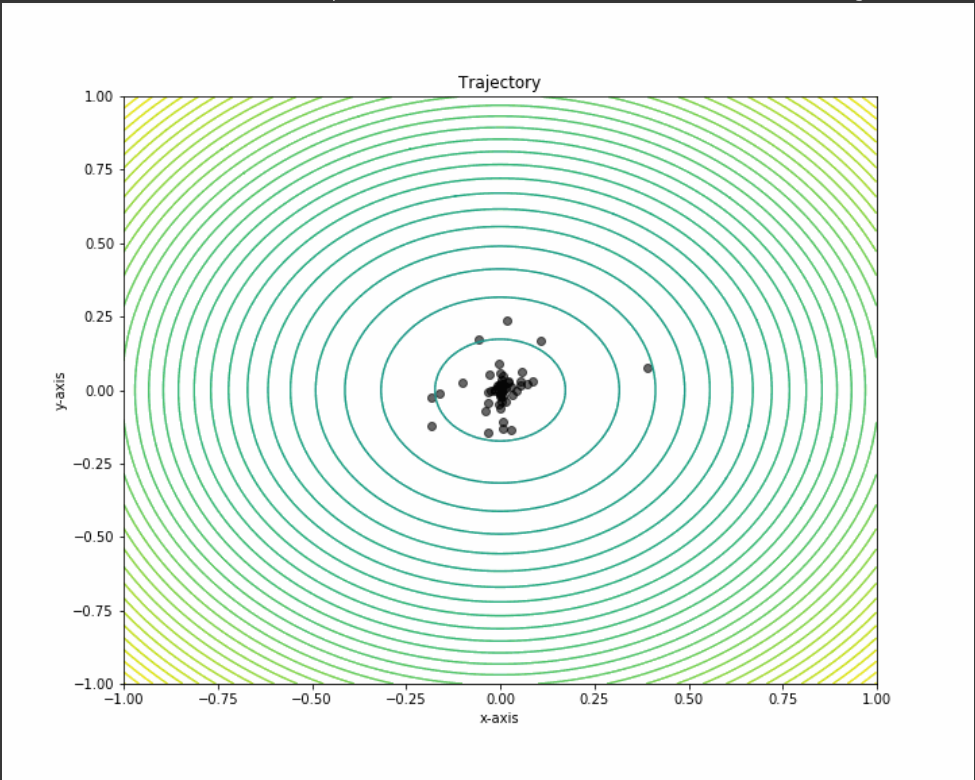
\includegraphics[width=0.5\textwidth]{images/pso2.png}
    \caption{PSO : Particles converging to global minima(Top view)}
\end{figure}
\subsubsection{Using PSO to solve Inverse Kinematics(IK) problem}
I was surprised when I came to know that same PSO can be applied to even solve the Inverse Kinematics problem in robotic manipulator. In general we use DH method to solve IK.\cite{dh}
Inverse Kinematics is the inverse function/algorithm of Forward Kinematics. The Forward Kinematics function/algorithm takes a target position as the input, and calculates the pose required for the end effector to reach the target position. While in inverse kinematics we find the joint value required for arm to reaches the given coordinate.
I use PSO (pyswarms library) to solve the IK, and detailed code for the same can be found \href{https://github.com/iamrajee/Slam_and_RL_BTP/tree/master/code/swarm/pso}{here}.
\newline \begin{figure}[H]
    \centering
    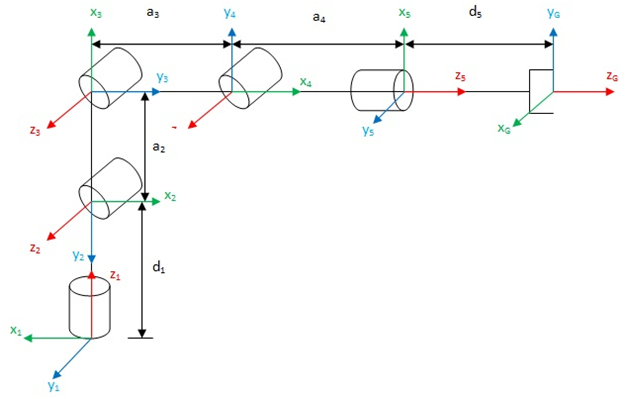
\includegraphics[width=0.8\textwidth]{images/6dof.jpg}
    \caption{IK : Finding inverse kinematics solution for 6 dof robotics manipulator}
\end{figure}

\subsubsection{Pseudo Code}
\begin{minted}{python}
# find forward kinematics pos of end effector
def get_end_tip_position(params):
    # Create the transformation matrices for the respective joints i.e find t_00, t_12, t_23, t_34, t_45,t_56

    # Get the overall transformation matrix
    end_tip_m = t_00.dot(t_01).dot(t_12).dot(t_23).dot(t_34).dot(t_45).dot(t_56)
    # The coordinates of the end tip are the 3 upper entries in the 4th column
    pos = np.array([end_tip_m[0,3],end_tip_m[1,3],end_tip_m[2,3]])
    return pos

# function to be optimized
def opt_func(X):
    n_particles = X.shape[0]  # number of particles
    target = np.array([-2,2,3])
    dist = [distance(get_end_tip_position(X[i]), target) for i in range(n_particles)]
    return np.array(dist)

# Call an instance of PSO
optimizer = ps.single.GlobalBestPSO(n_particles=swarm_size,
                                    dimensions=dim,
                                    options=options,
                                    bounds=constraints)

# Perform optimization
cost, joint_vars = optimizer.optimize(opt_func, iters=1000)
\end{minted}


\subsection{Flocking}
I used the ARGOS simulator to simulate the flocking behaviour(as described above) of ground robots. ARGOS is a open source simulation software, mostly popular for swarm robotics.\cite{argos} Here I spawn several robots in environment. Somewhere in the environment there is source of light. Each of the robot have the sensor to sense the light intensity. Based on this, flock of this robots tries to move towards light source. The detailed code for the same can be found \href{https://github.com/iamrajee/Slam_and_RL_BTP/tree/master/code/swarm/argos3-btp}{here}  and video of simulation can be found \href{https://youtu.be/y7pDO0bhHhA}{here}. 
\newline \begin{figure}[H]
    \centering
    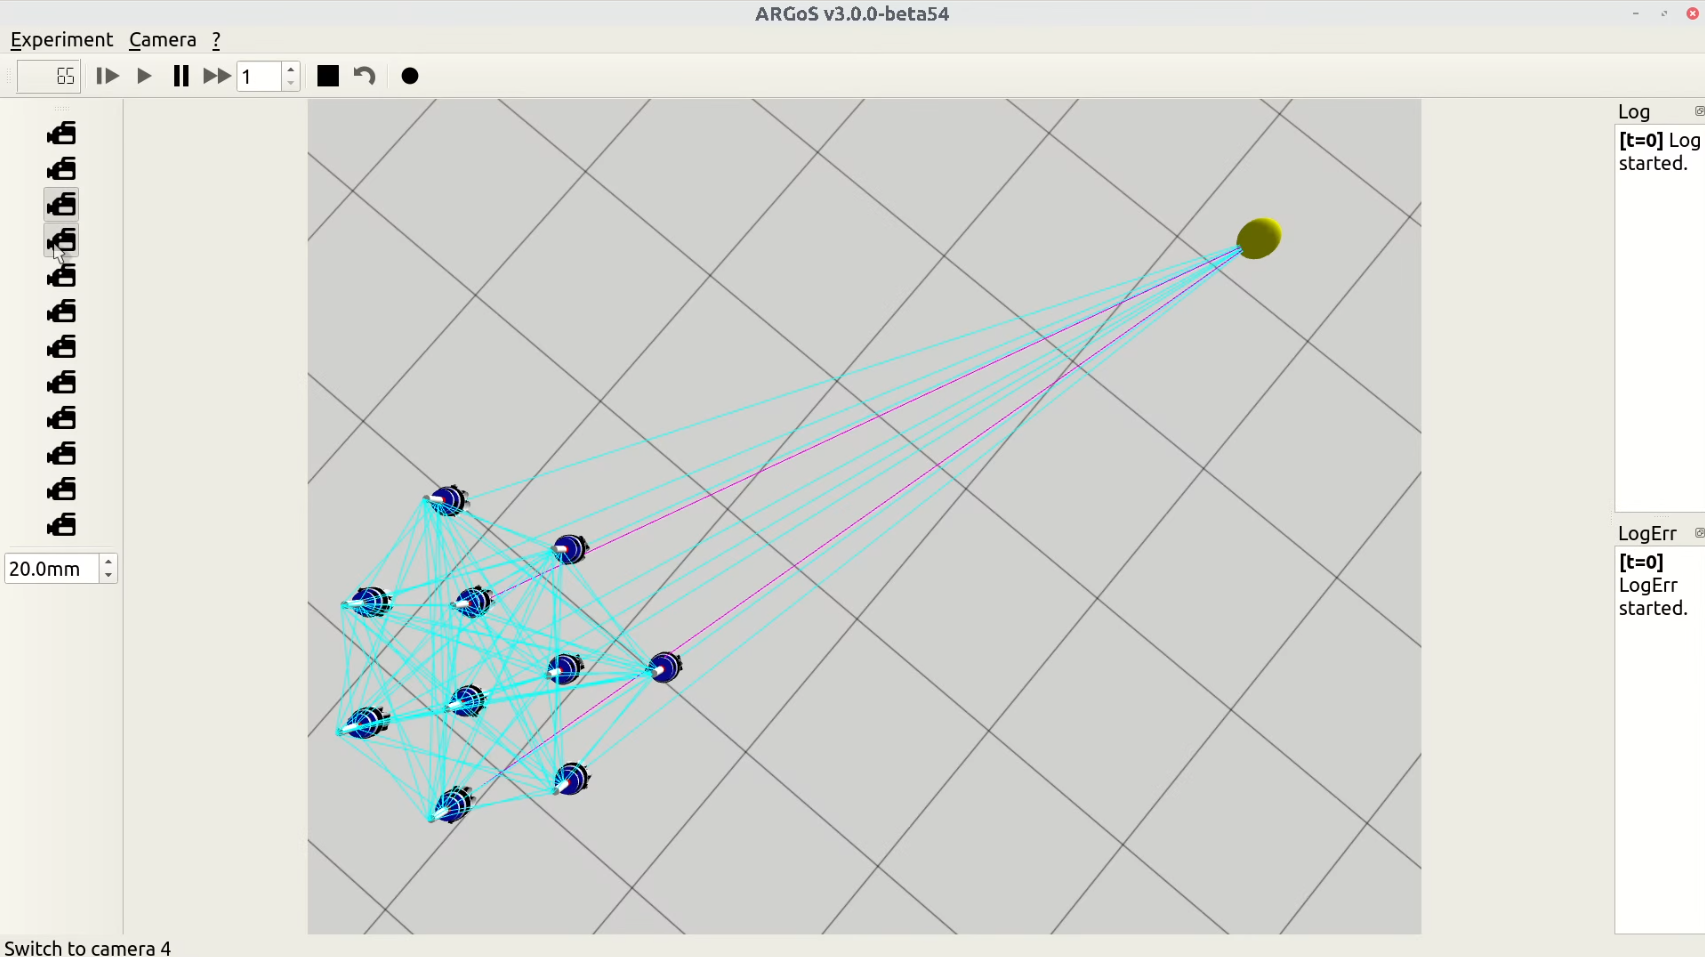
\includegraphics[width=0.8\textwidth]{images/flocking1.png}
    \caption{Robots started flocking towards light source}
\end{figure}
\newline \begin{figure}[H]
    \centering
    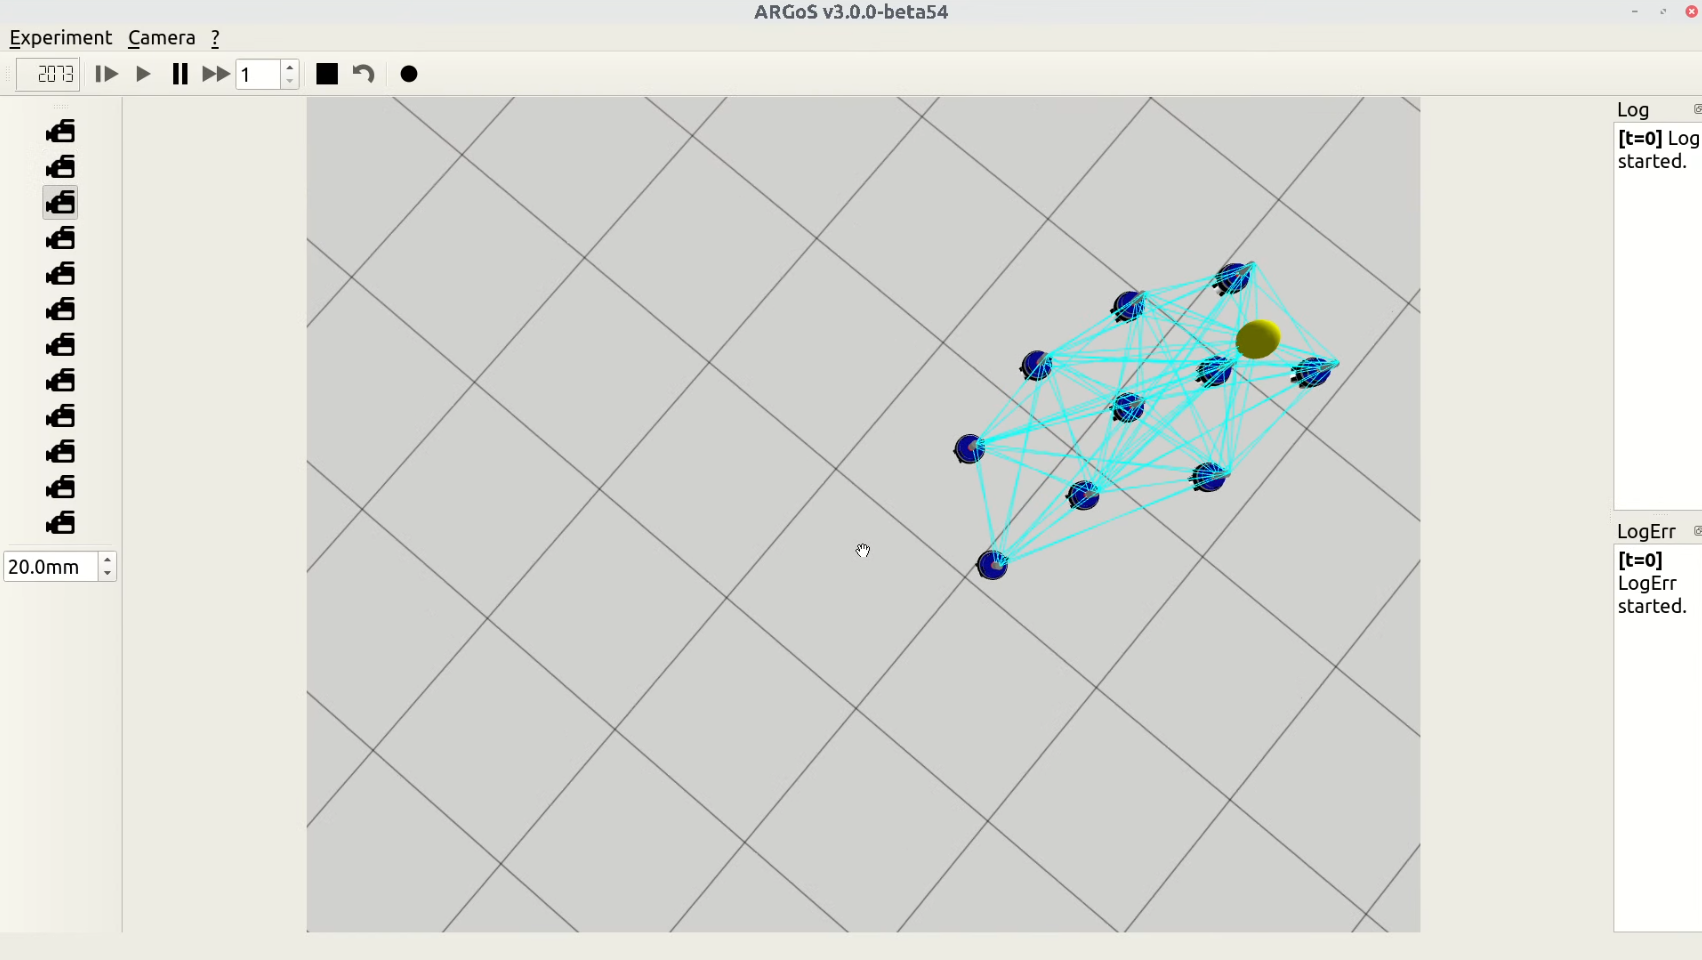
\includegraphics[width=0.8\textwidth]{images/flocking3.png}
    \caption{Robots flock almost reach light source}
\end{figure}

\subsubsection{Pseudo code}
\begin{minted}{c++}
 /* Get the camera readings */
 /* Go through the camera readings to calculate the flocking interaction vector */
 {
    for all blobs{     
        
        /*
          * The camera perceives the light as a yellow blob
          * The robots have their red beacon on
          * So, consider only red blobs
          * In addition: consider only the closest neighbors, to avoid
          * attraction to the farthest ones. Taking 180% of the target
          * distance is a good rule of thumb.
          */
         
        if color red && dist<target {
            /*
             * Take the blob distance and angle
             * With the distance, calculate the Lennard-Jones interaction force
             * Form a 2D vector with the interaction force and the angle
             * Sum such vector to the accumulator
             */
            /* Calculate LJ */
            /* Sum to accumulator */
            /* Increment the blobs seen counter */
        }
    }
    
    if(unBlobsSeen > 0) {
         /* Divide the accumulator by the number of blobs seen */
         /* Clamp the length of the vector to the max speed */
        /*Finally return flocking vecctor */
    }
}
\end{minted}


\subsection{Foraging}
Similar to flocking here we spawn several robots in environment in their nest(in some part of environment). Environment also contain food at several place. Now robot have to leave their nest, go out, find the food and pick it and bring it back into nest. The detailed code for the same can be found \href{https://github.com/iamrajee/Slam_and_RL_BTP/tree/master/code/swarm/argos3-btp}{here} and video of simulation can be found \href{https://youtu.be/kwznHmwixxc}{here}. 
\newline \begin{figure}[H]
    \centering
    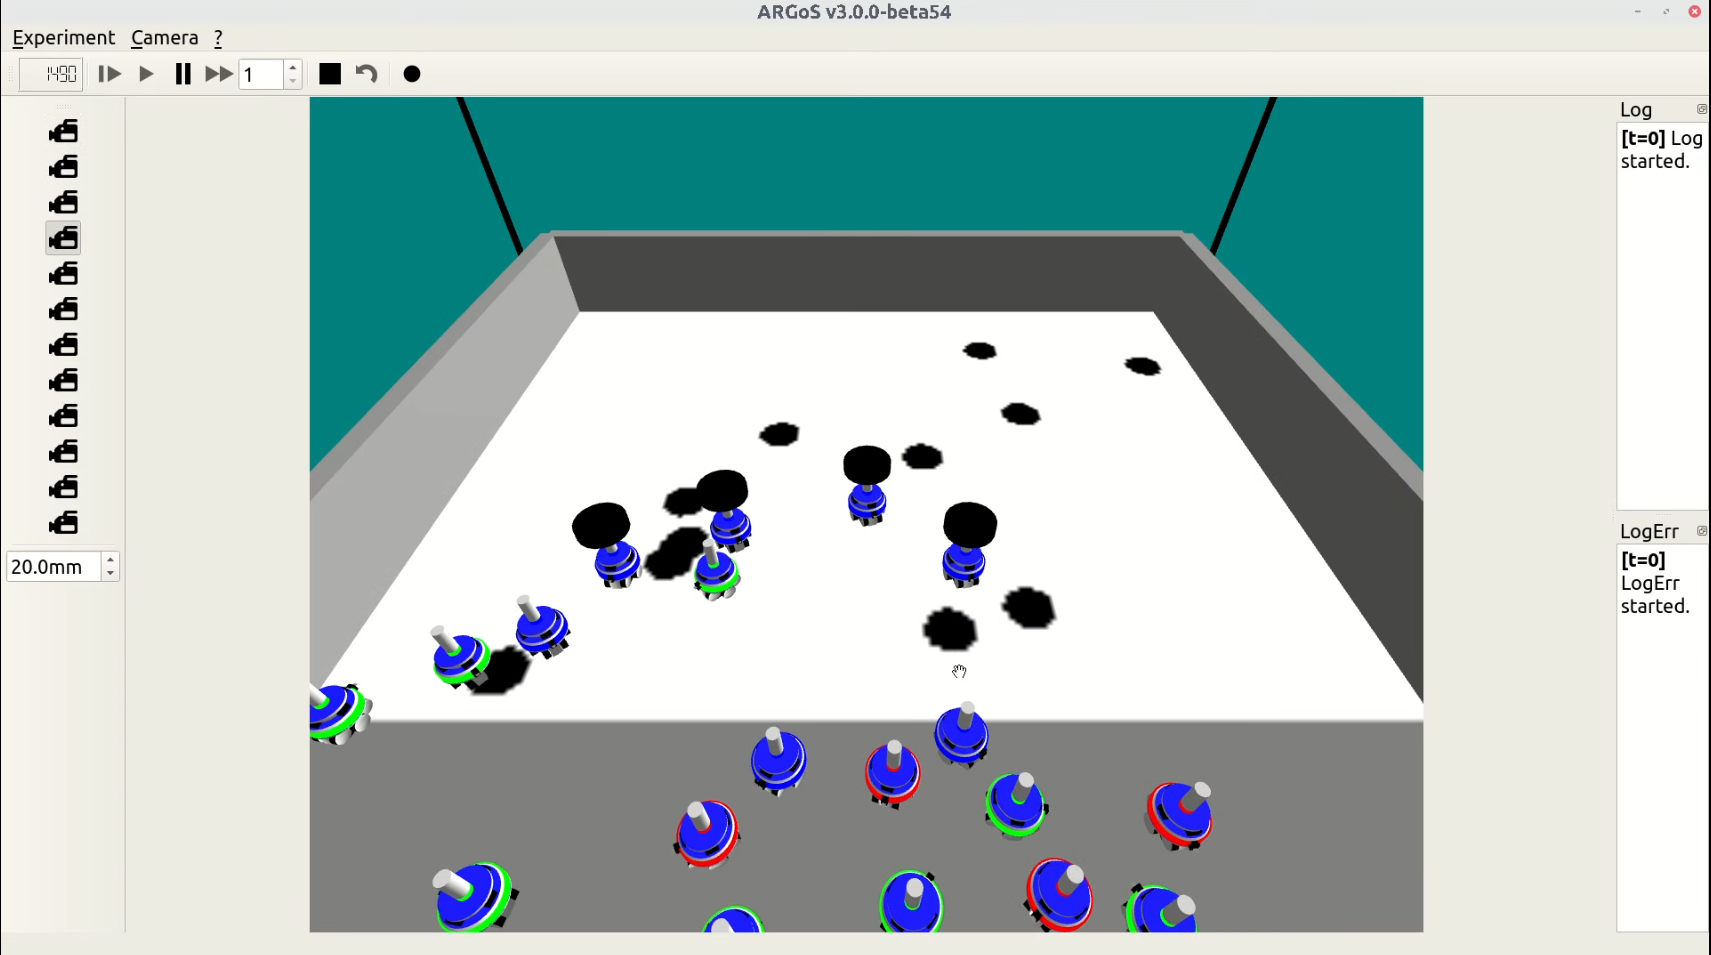
\includegraphics[width=0.8\textwidth]{images/foraging.png}
    \caption{Robots foraging for food source}
\end{figure}

\subsubsection{Pseudo code}
\begin{minted}{c++}
// ======================== UpdateState() ========================//
   /* Reset state flags */
   /* Read stuff from the ground sensor */
   /*
    * You can say whether you are in the nest by checking the ground sensor
    * placed close to the wheel motors. It returns a value between 0 and 1.
    * It is 1 when the robot is on a white area, it is 0 when the robot
    * is on a black area and it is around 0.5 when the robot is on a gray
    * area. 
    * The foot-bot has 4 sensors like this, two in the front
    * (corresponding to readings 0 and 1) and two in the back
    * (corresponding to reading 2 and 3).  Here we want the back sensors
    * (readings 2 and 3) to tell us whether we are on gray: if so, the
    * robot is completely in the nest, otherwise it's outside.
    */

// ==================== CalculateVectorToLight() ==================//
   /* Get readings from light sensor */
   /* Sum them together */
   /* If the light was perceived, return the vector */
   /* Otherwise, return zero */

// ==================== DiffusionVector() ===================//
   /* Get readings from proximity sensor */
   /* Sum them together */
   /* If the angle of the vector is small enough and the closest obstacle
      is far enough, ignore the vector and go straight, otherwise return it */
// ==================== SetWheelSpeedsFromVector() ===================//
   /* Get the heading angle */
   /* Get the length of the heading vector */
   /* Clamp the speed so that it's not greater than MaxSpeed */
   /* State transition logic */
   /* Wheel speeds based on current turning state */
   switch{
      case /* Just go straight */
      }
      case /* Both wheels go straight, but one is faster than the other */
      }
      case /* Opposite wheel speeds */
      }
   }
   /* Apply the calculated speeds to the appropriate wheels */
   /* Finally, set the wheel speeds */
   
   
// ==================== Explore() ===================//
/* We switch to 'return to nest' in two situations:
    * 1. if we have a food item
    * 2. if we have not found a food item for some time;
    *    in this case, the switch is probabilistic
    */
   /*
    * Test the first condition: have we found a food item?
    * NOTE: the food data is updated by the loop functions, so
    * here we just need to read it
    */
      /* Apply the food rule, decreasing ExploreToRestProb and increasing
       * RestToExploreProb */
      /* Store the result of the expedition */
      /* Switch to 'return to nest' */
   }
   /* Test the second condition: we probabilistically switch to 'return to
    * nest' if we have been wandering for some time and found nothing */
         /* Store the result of the expedition */
         /* Switch to 'return to nest' */
      }
      else {
         /* Apply the food rule, increasing ExploreToRestProb and
          * decreasing RestToExploreProb */
      }
   }
   /* So, do we return to the nest now? */
   if{
      /* Yes, we do! */
   }
   else {
      /* No, perform the actual exploration */
      /* Get the diffusion vector to perform obstacle avoidance */
      /* Apply the collision rule, if a collision avoidance happened */
         /* Collision avoidance happened, increase ExploreToRestProb and
          * decrease RestToExploreProb */
     /*
       * If we are in the nest, we combine antiphototaxis with obstacle
       * avoidance
       * Outside the nest, we just use the diffusion vector
       */
         /*
          * The vector returned by CalculateVectorToLight() points to
          * the light. Thus, the minus sign is because we want to go away
          * from the light.
          */
      }
      else {
         /* Use the diffusion vector only */
         
         
// ==================== ReturnToNest() ===================//
   /* As soon as you get to the nest, switch to 'resting' */
   /* Are we in the nest? */
     if{
      /* Have we looked for a place long enough? */
         /* Yes, stop the wheels... */
         /* Tell people about the last exploration attempt */
         /* ... and switch to state 'resting' */
      }
      else {
         /* No, keep looking */
      }
   }
   else {
      /* Still outside the nest */
   }
   /* Keep going */
// ==================== END ===================//
    
\end{minted}

\subsection{Synchronisation in the drone}
Here I want constrain two drones to fly place A to B in synchronisation. For this I use VREP and ROS. I spawn to two pluto drone in the VREP world. I used markers for localization of checkpoints of the path, obstacles and on the drones to locate them in the frame of an overhead camera which is watching this whole setup from the top. We used Aruco markers with different ids for obstacles and checkpoints of path. We also placed whycon markers on the drones to detect their position. Since the overhead camera is able to locate each of the markers in its frame of reference, both drones can now navigate on the predefined path synchronously while avoiding obstacles. PID control algorithm is used for drones to navigate between any two coordinates. We have to find such a path which can avoid obstacles and also navigate both drones maintaining their relative distance and attitude. For the same, I used Open Motion Planning Library(OMPL) on ROS and simulated the same in VREP. Here, we grouped both the drones and considered them as an object where only drones and obstacles were set as collidable. I use the OMPL algorithm to plan a path for midpoint of the group avoiding obstacles. Now, to get the individual path for both drones, firstly divided the midpoint path in some point called way-points. Now we found the initial offset of both drones from the mid-point in vector form, added it to each coordinate of midpoint path way-point. So, this way we are able to find the two separate paths for both the drones where distance between the drones is being maintained. So the only thing to be done now is to run both the drones on their corresponding path synchronously. We will give the way-points to the drone simultaneously. Suppose we have given the first pair of corresponding way-points to the drones. The next pair of way-points will be given only after both the drones reach their corresponding previous way-points properly. A point is said to be properly reached only if its error in all three axes is less than some given constant value.


\newline \begin{figure}[H]
    \centering
    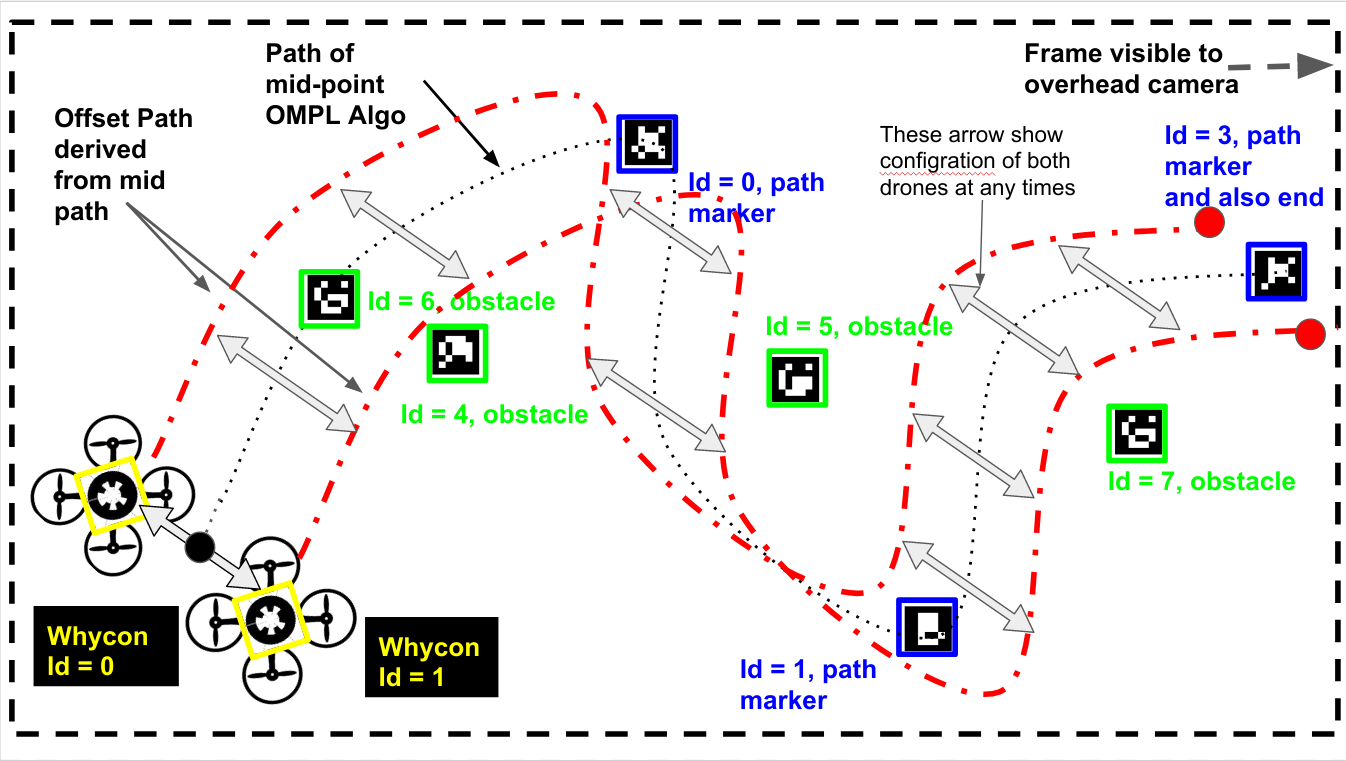
\includegraphics[width=0.8\textwidth]{images/plutoswarmAlgo.png}
    \caption{Algorithm flowchart for pluto drone synchronisation}
\end{figure}
\newline \begin{figure}[H]
    \centering
    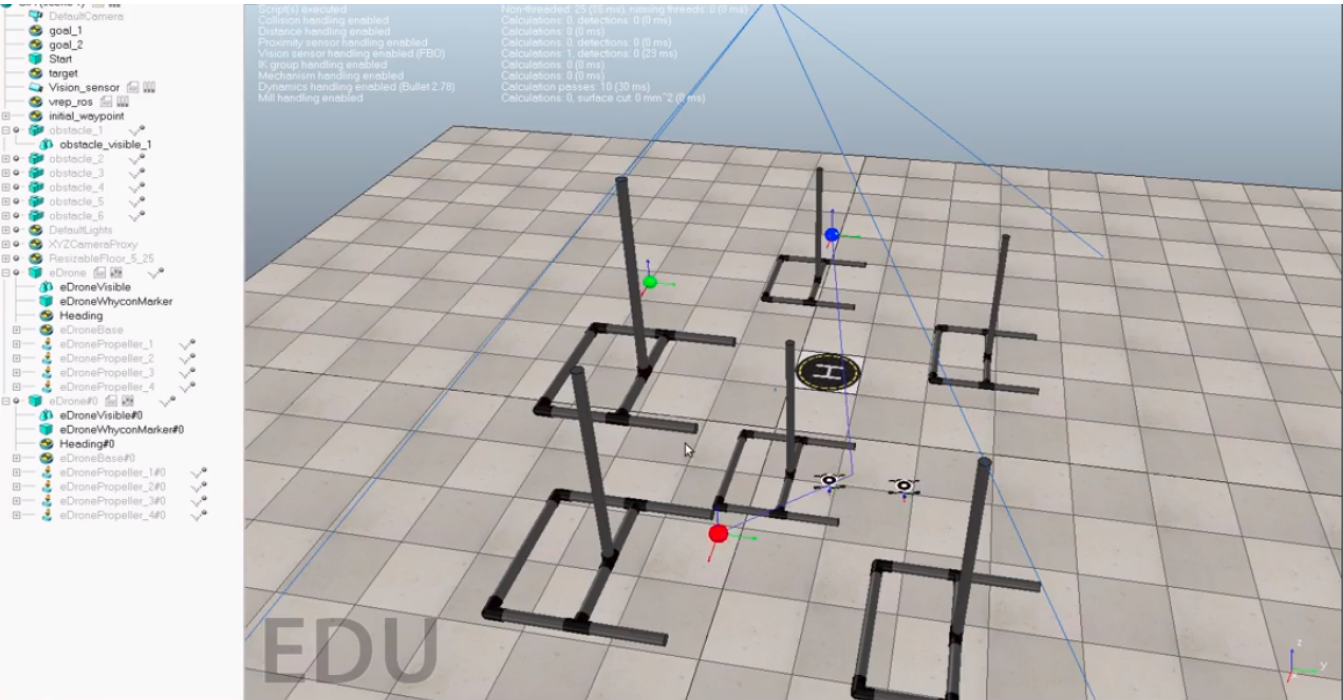
\includegraphics[width=0.8\textwidth]{images/plutoswarmVREP.png}
    \caption{VREP Simulation of above Algorithm}
\end{figure}

\subsection{Pseudo Code}
Once we get the list of set point(using above algorithm) for both the drone rest code very much similar to one used in section 4.1.2.
\begin{minted}{python}
'''
Code only here as below
'''
if __name__ == '__main__':
    pid_class = PID() #pid class as described in previous pid controller code
    error = []
    while True:
        error = pid_class.pid(pid_class.initialSetPoint)
        if (abs(error[0]) <= 0.5 and abs(error[1]) <= 0.5 and abs(error[2]) <= 0.5):
            break
    for i in range (0, 3):
        if i != 0:
            print("next_target")
        pid_class.next.publish('1')
        rospy.sleep(0.5)
        length = len(pid_class.setPoint.poses)
        for j in range (0, length):
            temp = [0.0, 0.0, 0.0, 0.0]
            temp[0] = pid_class.setPoint.poses[j].position.x
            temp[1] = pid_class.setPoint.poses[j].position.y
            temp[2] = pid_class.setPoint.poses[j].position.z
            temp[3] = 0.0
            while (True):
                error = pid_class.pid(temp)
                if (error[0] <= 0.5 and error[1] <= 0.5 and error[2] <= 0.5):
                    break
    # pid_class.disarm()

    #land at start point
    while True:
        error = pid_class.pid(pid_class.start)
        if (abs(error[0]) <= 0.5 and abs(error[1]) <= 0.5 and abs(error[2]) <= 1):
            pid_class.disarm()
            break
\end{minted}


\section{Conclusion}
This chapter we studied swarm behaviour of robot in depth and how it can help a group as whole to benefit from each other. We also implemented flocking, foraging and pso in code.
% hi \cite{Omar2016}
% bye \cite{WikiFlocking}